\documentclass[draft]{article}

% if you need to pass options to natbib, use, e.g.:
% \PassOptionsToPackage{numbers, compress}{natbib}
% before loading nips_2016
%
% to avoid loading the natbib package, add option nonatbib:
% \usepackage[nonatbib]{nips_2016}

\usepackage{nips_2016}

\usepackage{amsmath} % used for matrices in math mode

% to compile a camera-ready version, add the [final] option, e.g.:
% \usepackage[final]{nips_2016}

\usepackage[utf8]{inputenc} % allow utf-8 input
\usepackage[T1]{fontenc}    % use 8-bit T1 fonts
\usepackage{hyperref}       % hyperlinks
\usepackage{url}            % simple URL typesetting
\usepackage{booktabs}       % professional-quality tables
\usepackage{amsfonts}       % blackboard math symbols
\usepackage{nicefrac}       % compact symbols for 1/2, etc.
\usepackage{microtype}      % microtypography
\usepackage{textcomp}

\usepackage{graphicx}  % Required for including images

\usepackage{subcaption}
\captionsetup{compatibility=false}

\bibliographystyle{dcu}

\title{Pre-Training CNN's Using Convolutional Autoencoders}

% The \author macro works with any number of authors. There are two
% commands used to separate the names and addresses of multiple
% authors: \And and \AND.
%
% Using \And between authors leaves it to LaTeX to determine where to
% break the lines. Using \AND forces a line break at that point. So,
% if LaTeX puts 3 of 4 authors names on the first line, and the last
% on the second line, try using \AND instead of \And before the third
% author name.

\author{
  David S.~Hippocampus\thanks{Use footnote for providing further
    information about author (webpage, alternative
    address)---\emph{not} for acknowledging funding agencies.} \\
  Department of Computer Science\\
  Cranberry-Lemon University\\
  Pittsburgh, PA 15213 \\
  \texttt{hippo@cs.cranberry-lemon.edu} \\
  %% examples of more authors
  %% \And
  %% Coauthor \\
  %% Affiliation \\
  %% Address \\
  %% \texttt{email} \\
  %% \AND
  %% Coauthor \\
  %% Affiliation \\
  %% Address \\
  %% \texttt{email} \\
  %% \And
  %% Coauthor \\
  %% Affiliation \\
  %% Address \\
  %% \texttt{email} \\
  %% \And
  %% Coauthor \\
  %% Affiliation \\
  %% Address \\
  %% \texttt{email} \\
}

\begin{document}
% \nipsfinalcopy is no longer used

\maketitle

\begin{abstract}
  We are comparing the effect of pretraining.
\end{abstract}

\section{Introduction}
\section{Related Work}
Masci et. al (2011) introduced the Convolutional Auto-Encoder, an unsupervised method for hierarchical feature extraction, which learns biologically plausible filters. Masci et. al demonstrated that a CNN can be initialized by a CAE stack. Although CAE’s overcomplete hidden representation makes learning harder,  interesting and visually nicest filters emerge if a max-pooling layer is used. They experimented with twenty 7 x 7 filters of four CAEs of the same topology, and trained them differently on MNIST dataset. The first one of the CAEs was trained on original digits, the second one on noisy inputs with 50\% binomial noise added, the third one with an additional max-pooling layer of size 2 x 2 and the fourth one on noisy (30\% binomial noise) inputs with a max-pooling layer of size 2 x 2. When they compared the results, it turned out that interesting and biologically plausible filters emerged only when the CAE is trained with a max-pooling layer. When the CAE is trained without any additional constraints, it learned trivial solutions and when they trained the CAE with additional noise, it became more localized. They repeated the above experiment on CIFAR10 dataset and found striking impact of a max-pooling layer whereas adding noise had almost no visual effect except on the weight magnitudes, indicating that max-pooling is essential. They also demonstrated that pre-trained CNNs consistently outperform randomly initialized CNN.

Hamester et. al (2015) proposed a model using a variant of the Multi-channel Convolutional Neural Network for face expression recognition which does not depend on any hand-crafted or task specific feature extraction but exploits unsupervised learning, using a multiple CNNs based 2-channel architecture, where the CNNs first process information independently and then all streams merge in a fully connected layer, which is used for classification. The wights of the channel were trained as convolutional auto-encoder (CAE). They evaluated the model on JAFFE dataset and found that the model is a very viable method for facial expression recognition. They easily reached the state-of-the-art recognition rates with minimal effort and achieved an average of 95.8\% accuracy which was 8.1\% higher than the previous state-of-the-art (Sumbramaniam et. al (2012)).
\section{Setup \& Context}
  
  In this paper, we evaluate the influence of CNN pre-training using convolutional autoencoders on the network's out-of-sample accuracy. To achieve this, we train, in a first step, a convolutional autoencoder on a chosen dataset and then, in a second step, use it's convolution layer weights to initialize the convolution layers of a CNN. After training, we compare the CNN's test set accuracy to a reference network that was trained under the same conditions with randomly initialized convolution weights. 

  \begin{figure}[h]
    \centering
    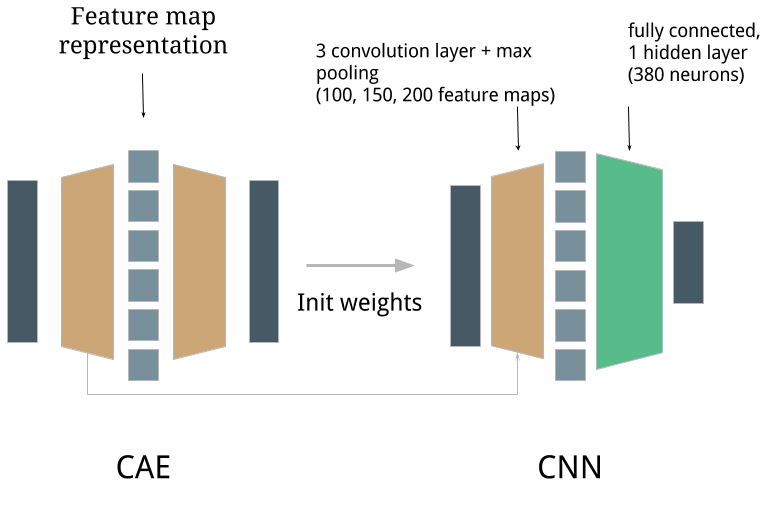
\includegraphics[width=0.5\linewidth]{../graphics/setup.png}
    \caption{Experimental Setup}
    \label{fig:experimental_setup}
  \end{figure}

  A visualization of the weight transfer can be seen on the schematic in figure ~\ref{fig:experimental_setup}. 

  \begin{itemize}
    \item CAE on full / CNN on part of the data (expensive labels scenario)
  \end{itemize}

  \subsection{Autoencoder Architecture + Training}

    \paragraph{Architecture}
    The convolutional autoencoder first uses several convolution layers and pooling layers to transform the input to a feature map representation and then reconstructs the input using strided transposed convolutions (TODO: similar to Zeiler / first GAN layers? + citation). In our experiments, the encoding part consisted of:

    in general: conv layers have (1,1,1,1) strides and we are performing a full convolution (out hei/wid = in hei(wid))

    input (batchsize, height, width, numchannels) -> conv1 (5x5 filter) (batchsize, height, width, 100) -> activation function (scaled tanh) (b,h,w,100) -> max pooling (2x2, (1,2,2,1) strides) (b, h/2, w/2, 100) -> conv2 (5x5 filter) (b, h/2, w/2, 150) -> activation function (Scaled tanh) (b, h/2, w/2, 150) -> max  pooling (2x2 filter, (1,2,2,1) strides (b, h/4, w/4, 150) -> conv3 (3x3 filter), (b, h/4, w/4, 200) -> activation function (scaled tanh) (b, h/4, w/4, 200) 

    \begin{itemize}
      \item Upsampling + Reconstruction
    \end{itemize}

    \paragraph{Activation Function} We tried 3 different activations (sigmoid, scaled tanh and relu). For our main experiments, we decided on the the scaled tanh as used in (TODO: add citation). We will talk about our ReLU experiments in (TODO: add link). With scaled tanh we mean the tanh function rescaled and shifted to the [0,1] output range. This corresponds to the function $$scaledtanh(x) = \frac{1}{2}tanh(x) + \frac{1}{2}$$ which has a generally sigmoidal shape but a stronger gradient around $x = 0$. In our experiments, CAEs seemed faster to train using this function, however we did not conduct any experiments to verify this.

    \paragraph{Regularization} In general, a full convolutional layer could easily learn a simple point filter such as $k = \begin{smallmatrix} 0&0&0\\ 0&1&0 \\ 0&0&0 \end{smallmatrix}$ (for 1d input) that copies the input onto a feature map. While this would later simplify a perfect reconstruction of the input, the CAE did not find any more suitable representation for our data. To prevent this problem, some kind of regularization is needed, several methods can be found in the literature, most of them involving some kind of sparsity constraint for the representation layer (TODO: reference sparse CAE paper and more regularization ideas?). In (TODO: cite stacked conv auto), the authors use max-pooling as an elegant way to enforce the learning of plausible filters without the need for any further regularization. Since the CNN architecture we are going to use later will contain pooling layers anyways, we sticked with this technique and chose not to add any noise to our inputs either since this seemed not to help the emergence of more natural filters. (TODO: describe what is a natural filter for us). 

    \paragraph{Training} While (TODO: add citations) used a layer-wise training for convolutional autoencoders, we achieved good results by training the whole auto-encoder at once. (TODO: maybe this made it more difficult / longer to train?). For the \emph{MNIST} and \emph{CIFAR-10} datasets, the autoencoders were trained with simple gradient descent using as learning rate of $lr = 0.5$ (TODO: VERIFY THAT!), for the CKPLUS dataset, we used the adagrad optimizer with the same initial learning rate $lr$. (TODO:VERIFY THAT!)


    \paragraph{Weight initialization} The convolutional filters were initialized using a truncated normal distribution with mean $\mu = 0.001$ and standard deviation $\sigma = 0.05$, all bias values were initialized with the constant $0.001$

  \subsection{Pre-Training and Test Methodology}

    \paragraph{CNN architecture} The CNN uses the same architecture as the CAE encoding for its convolution layers (feature extraction) and then uses a fully-connected layer with size 384 followed by an activation function (scaled tanh), a second fully-connected layer of size 10 and a softmax layer for classification. 

    \paragraph{Weight Initialization}

    The convolutional layer weights (filters) and biases of the pre-trained networks were initialized with the values obtained from the convolutional autoencoders.

    The reference CNN's convolution weights were initialized with mean $\mu = 0 $ and standard deviation $\sigma = 0.2$, the biases with the constant value $b =  0.0001$.

    The fully-connected layers were initialized randomly for all networks, the weights with a truncated normal distribution with mean $\mu = 0$ and standard deviation $\sigma = 0.001$ and the biases with the constant value $0.0001$.
    This means that for all experiments, some parts of the networks are randomly initialized, all weights for the reference networks and the fully-connected weights for the pre-trained networks. 

    \paragraph{CNN Training}
    (TODO: optimizer, step size, convergence criterion, amount of epochs per dataset)

    For each datset, we split the available training data into training and evaluation set and used the evaluation set to track the training progress and adjust hyperparameters. We kept track of both cross-entropy error and accuracy on the evaluation set and stopped training when these values converged. Afterwards, we evaluated the networks accuracy once on the held-out test set and used the obtained value as a result. 

    For the larger datasets \emph{MNIST} and \emph{CIFAR-10}, we conducted several experiments restricting the amount of available training data inspired by (TODO: cite stacked conv autoencoders). The autoencoder used for pre-training was always trained on the whole dataset. 

    %\begin{itemize}
      %\item Network Architectures
      %\item Weight Transfer
      %\item weight initialization (all layers)
      %\item CNN Training
      %\item Test Methodology (Train + Validation + Test Sets)
      %\item 1k/10k/full splits but always full dataset for CAE
    %\end{itemize}

  \subsection{Evaluation}
    For each dataset and training size, we trained (TODO adjust to real number) k pre-trained CNNs and k randomly initialized reference CNNs. (TODO: add significance test?)
  

\section{Experiments}
  % Results and challenges while performing experiments
  % Training process
  % How long trained
  % convergence criterion (checked how long they took)
  % amount of epochs per dataset
  % evaluated on test set
  % shrink boxplots, next to each other
  % FOCUS: CK+ Processing

  \subsection{Datset Descriptions and Challenges}
  We conducted experiments on three different datasets, which vary in their image size, number of images and colour information.
    \subsubsection{MNIST}
        \begin{figure}[h]
          \centering
          
\includegraphics[width=0.15\linewidth]{../graphics/reconstructions/mnist/input_00.png}
          
\includegraphics[width=0.15\linewidth]{../graphics/reconstructions/mnist/input_01.png}
          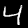
\includegraphics[width=0.15\linewidth]{../graphics/reconstructions/mnist/input_02.png}

          
\includegraphics[width=0.15\linewidth]{../graphics/reconstructions/mnist/reconstruction_00.png}
          
\includegraphics[width=0.15\linewidth]{../graphics/reconstructions/mnist/reconstruction_01.png}
          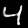
\includegraphics[width=0.15\linewidth]{../graphics/reconstructions/mnist/reconstruction_02.png}

          \caption{\emph{MNIST} example images (top) and CAE reconstructions (bottom)}
        \end{figure}
        MNIST \citep{lecun1998mnist} is the standard dataset used for image classification. It consists of scanned handwritten digits, which are 28 by 28 pixel grayscale images.
    \subsubsection{CIFAR-10}
    	\begin{figure}[h]
        \centering
        %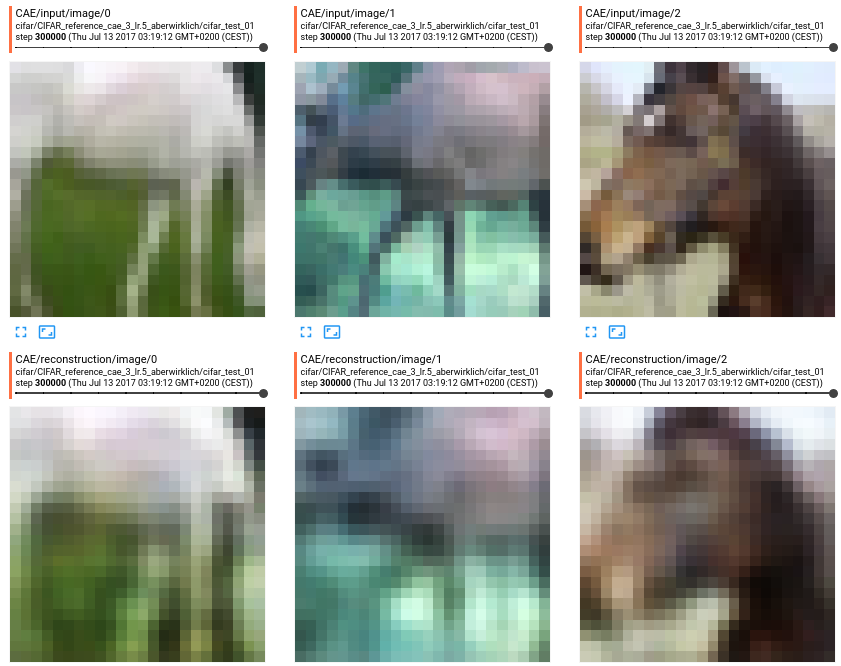
\includegraphics[width=0.8\linewidth]{../graphics/cifar_reconstructions.png}
        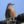
\includegraphics[width=0.2\linewidth]{../graphics/reconstructions/cifar/input_00.png}
        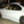
\includegraphics[width=0.2\linewidth]{../graphics/reconstructions/cifar/input_01.png}
        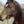
\includegraphics[width=0.2\linewidth]{../graphics/reconstructions/cifar/input_02.png}

        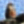
\includegraphics[width=0.2\linewidth]{../graphics/reconstructions/cifar/reconstruction_00.png}
        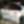
\includegraphics[width=0.2\linewidth]{../graphics/reconstructions/cifar/reconstruction_01.png}
        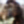
\includegraphics[width=0.2\linewidth]{../graphics/reconstructions/cifar/reconstruction_02.png}

        \caption{\emph{CIFAR-10} example images(top) and CAE reconstructions(bottom)}

      \end{figure}
      The CIFAR dataset \citep{krizhevsky2009learning} is made out of natural scenes, which are 32x32 colorized images. The relatively low resolution, while still and the colors lead to a more complex
      The CIFAR-10 variant, which we used, is built as a classification dataset with 10 specified labels (cars, cats...)
    \subsubsection{CK+}
    \textbf{if I reproduce images in electronic or print media, to use only those from the following subjects 
S52, S55, S74, S106, S111, S113, S121, S124, S125, S130, S132} \\
      \begin{figure}[h]
        \centering
        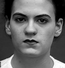
\includegraphics[width=0.2\linewidth]{../graphics/reconstructions/ckplus/input_00.png}
        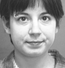
\includegraphics[width=0.2\linewidth]{../graphics/reconstructions/ckplus/input_01.png}
        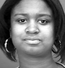
\includegraphics[width=0.2\linewidth]{../graphics/reconstructions/ckplus/input_02.png}

        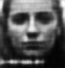
\includegraphics[width=0.2\linewidth]{../graphics/reconstructions/ckplus/reconstruction_00.png}
        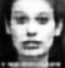
\includegraphics[width=0.2\linewidth]{../graphics/reconstructions/ckplus/reconstruction_01.png}
        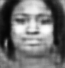
\includegraphics[width=0.2\linewidth]{../graphics/reconstructions/ckplus/reconstruction_02.png}

        %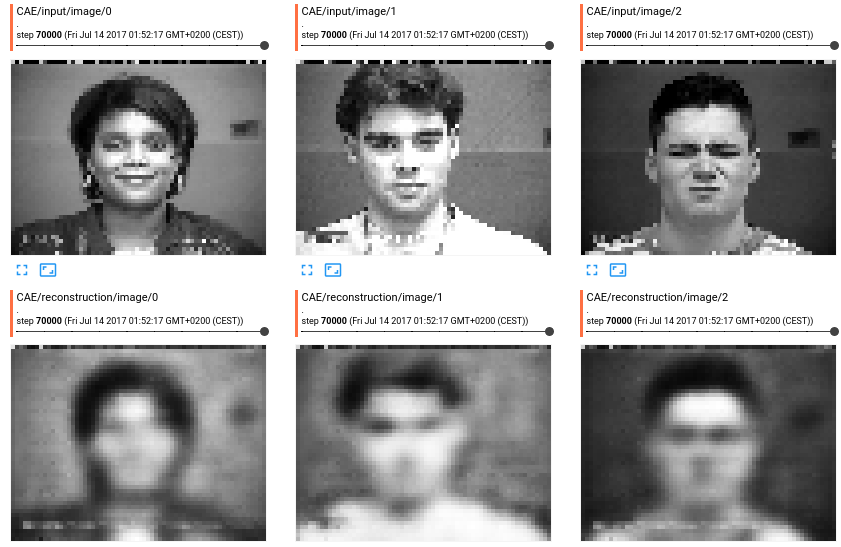
\includegraphics[width=0.8\linewidth]{../graphics/ckplus_reconstructions_better.png}
        \caption{CK+ input image (top) and reconstruction (bottom) ({\textcopyright}Jeffrey Cohn)}
      \end{figure}
      The Extended Cohn-Kanade (CK+) dataset \citep{kanade2000comprehensive,lucey2010extended} was the most interesting dataset during our project.
      Unlike the other two datasets, no pre-training experiments have been done on CK+, as far as we know.
      As the CK+ dataset is not readily prepared for running those kinds of experiments, we had to put some work into this ourselves.
      We decided to not take the full images, but used the provided facial landmarks, to put the faces into a bounding box and scale them down by factor 5 to a size of 68x65 pixels.
      Alltogether CK+ has 123 subjects and 593 emotion sequences, which are 10-60 frames of short video sequences, from a neutral face to the target emotion.
      In order to train the autoencoder we used all of the frames as unlabelled input, for the CNN we used the last three frames of all sequences, labelled with the target emotion.
      We split the dataset into training, validation and test set by subject, so that we end up with 696 training, 87 validation and 198 test images.
      Before training we randomly shuffle the images.

  \subsection{Autoencoder Training}
    For the autoencoder training we took each of the three datasets' images, reshaped them into a vector and used these values as input and target output for a convolutional autoencoder. The architecture for the autoencoder was chosen in a way, so that the CNN would give best results.

    For the loss function we decided to use the mean-squared error, as cross-entropy did not give us good results. % Maybe add explanation? Only if enough time


    \subsubsection{ReLu activation function}
      In further experiments we used the ReLu activation function \citep{nair2010rectified} for the autoencoder.
      This lead to quite good-looking representations, while the filters did not seem to have much structure, see figure \ref{fig:relu_cae}.

      \begin{figure}[h]

				\begin{subfigure}{0.4\linewidth}

					\centering
					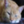
\includegraphics[width=0.4\linewidth]{../graphics/reconstructions/cifar/relu/input_00_relu.png}
					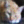
\includegraphics[width=0.4\linewidth]{../graphics/reconstructions/cifar/relu/reconstruction_00_relu.png}
					%\caption{(CAE:) Reconstruction example using ReLU activation + smaller network size}

				\end{subfigure}
				\begin{subfigure}{0.4\linewidth}

					\centering
					
\includegraphics[width=0.1\linewidth]{../graphics/reconstructions/cifar/relu/relu_filter_00.png} \hspace{0.05\linewidth}
					
\includegraphics[width=0.1\linewidth]{../graphics/reconstructions/cifar/relu/relu_filter_01.png} \hspace{0.05\linewidth}
					
\includegraphics[width=0.1\linewidth]{../graphics/reconstructions/cifar/relu/relu_filter_02.png} \\
					\vspace{0.05\linewidth}
					
\includegraphics[width=0.1\linewidth]{../graphics/reconstructions/cifar/relu/relu_filter_03.png} \hspace{0.05\linewidth}
					
\includegraphics[width=0.1\linewidth]{../graphics/reconstructions/cifar/relu/relu_filter_04.png} \hspace{0.05\linewidth}
					
\includegraphics[width=0.1\linewidth]{../graphics/reconstructions/cifar/relu/relu_filter_05.png} \\
					\vspace{0.05\linewidth}
					
\includegraphics[width=0.1\linewidth]{../graphics/reconstructions/cifar/relu/relu_filter_06.png} \hspace{0.05\linewidth}
					
\includegraphics[width=0.1\linewidth]{../graphics/reconstructions/cifar/relu/relu_filter_07.png} \hspace{0.05\linewidth}
					
\includegraphics[width=0.1\linewidth]{../graphics/reconstructions/cifar/relu/relu_filter_08.png} 

					%\caption{(CAE:) Structureless first layer filters learned by ReLU autoencoder}

				\end{subfigure}

			\caption{\textbf{ReLU CAE} example input + reconstruction (left), selection of first layer filters (right) }
			\label{fig:relu_cae}

    \end{figure}

  \subsection{Pretraining and Classification}
    The general idea of pretraining a classification neural network, is to transfer the encoding weights of the CAE to the CNN. So we took the convolutional filter weights, which we generated during the autoencoder training, and used them as initial values for the convolutional layers for the classification network.

    As the MNIST and CIFAR-10 datasets consist of a lot more images than CK+, we decided to follow the approach of the paper and take a 1k and 10k subset for these two. So while we still took all training images for building a decent autoencoder, the CNN could only use some of the images. This is especially interesting to check the hypothesis, that pre-training makes more sense, when you have less training images.

    To validate our pretraining experiments, in each run we set up a CNN with randomly initialized filters and a CNN which uses the filters trained by the CAE. Both networks have randomly initialized weights for their dense layers.

    We let all networks run for at least x (TODO) epochs for all datasets, until the MSE did not change significantly anymore.

    After the final training we measured the classification accuracy on the separate testset, so that we can measure generalization.
      % Training process
      % evaluated on test set
    \subsubsection{Interpretation}
      For all datasets it can be observed, that the accuracy on a pre-trained CNN is higher than with a randomly initialized CNN, when we use the full or 10k datasets.
      For the 1k subsets of MNIST and CIFAR-10, no significant improvement seems to occur. This could
      be due to overfitting, as we train a complex network on very little data.
      For the CK+ dataset we get the biggest improvement through pretraining.
      Even though the standard deviation is quite high, we get a significant jump in the accuracy.
      This could be due to the fact, that for CK+ we use all, including neutral and ambiguous, frames (5876 images) to train the CAE, so that the pre-trained filters have more material to learn features from.
      % Should we write this into Conclusion: ?
      This leads to the conclusion, that pretraining is espcially applicable, when there are much more unlabbeled images but only a few that can be used for learning classifications.

    \begin{figure}
      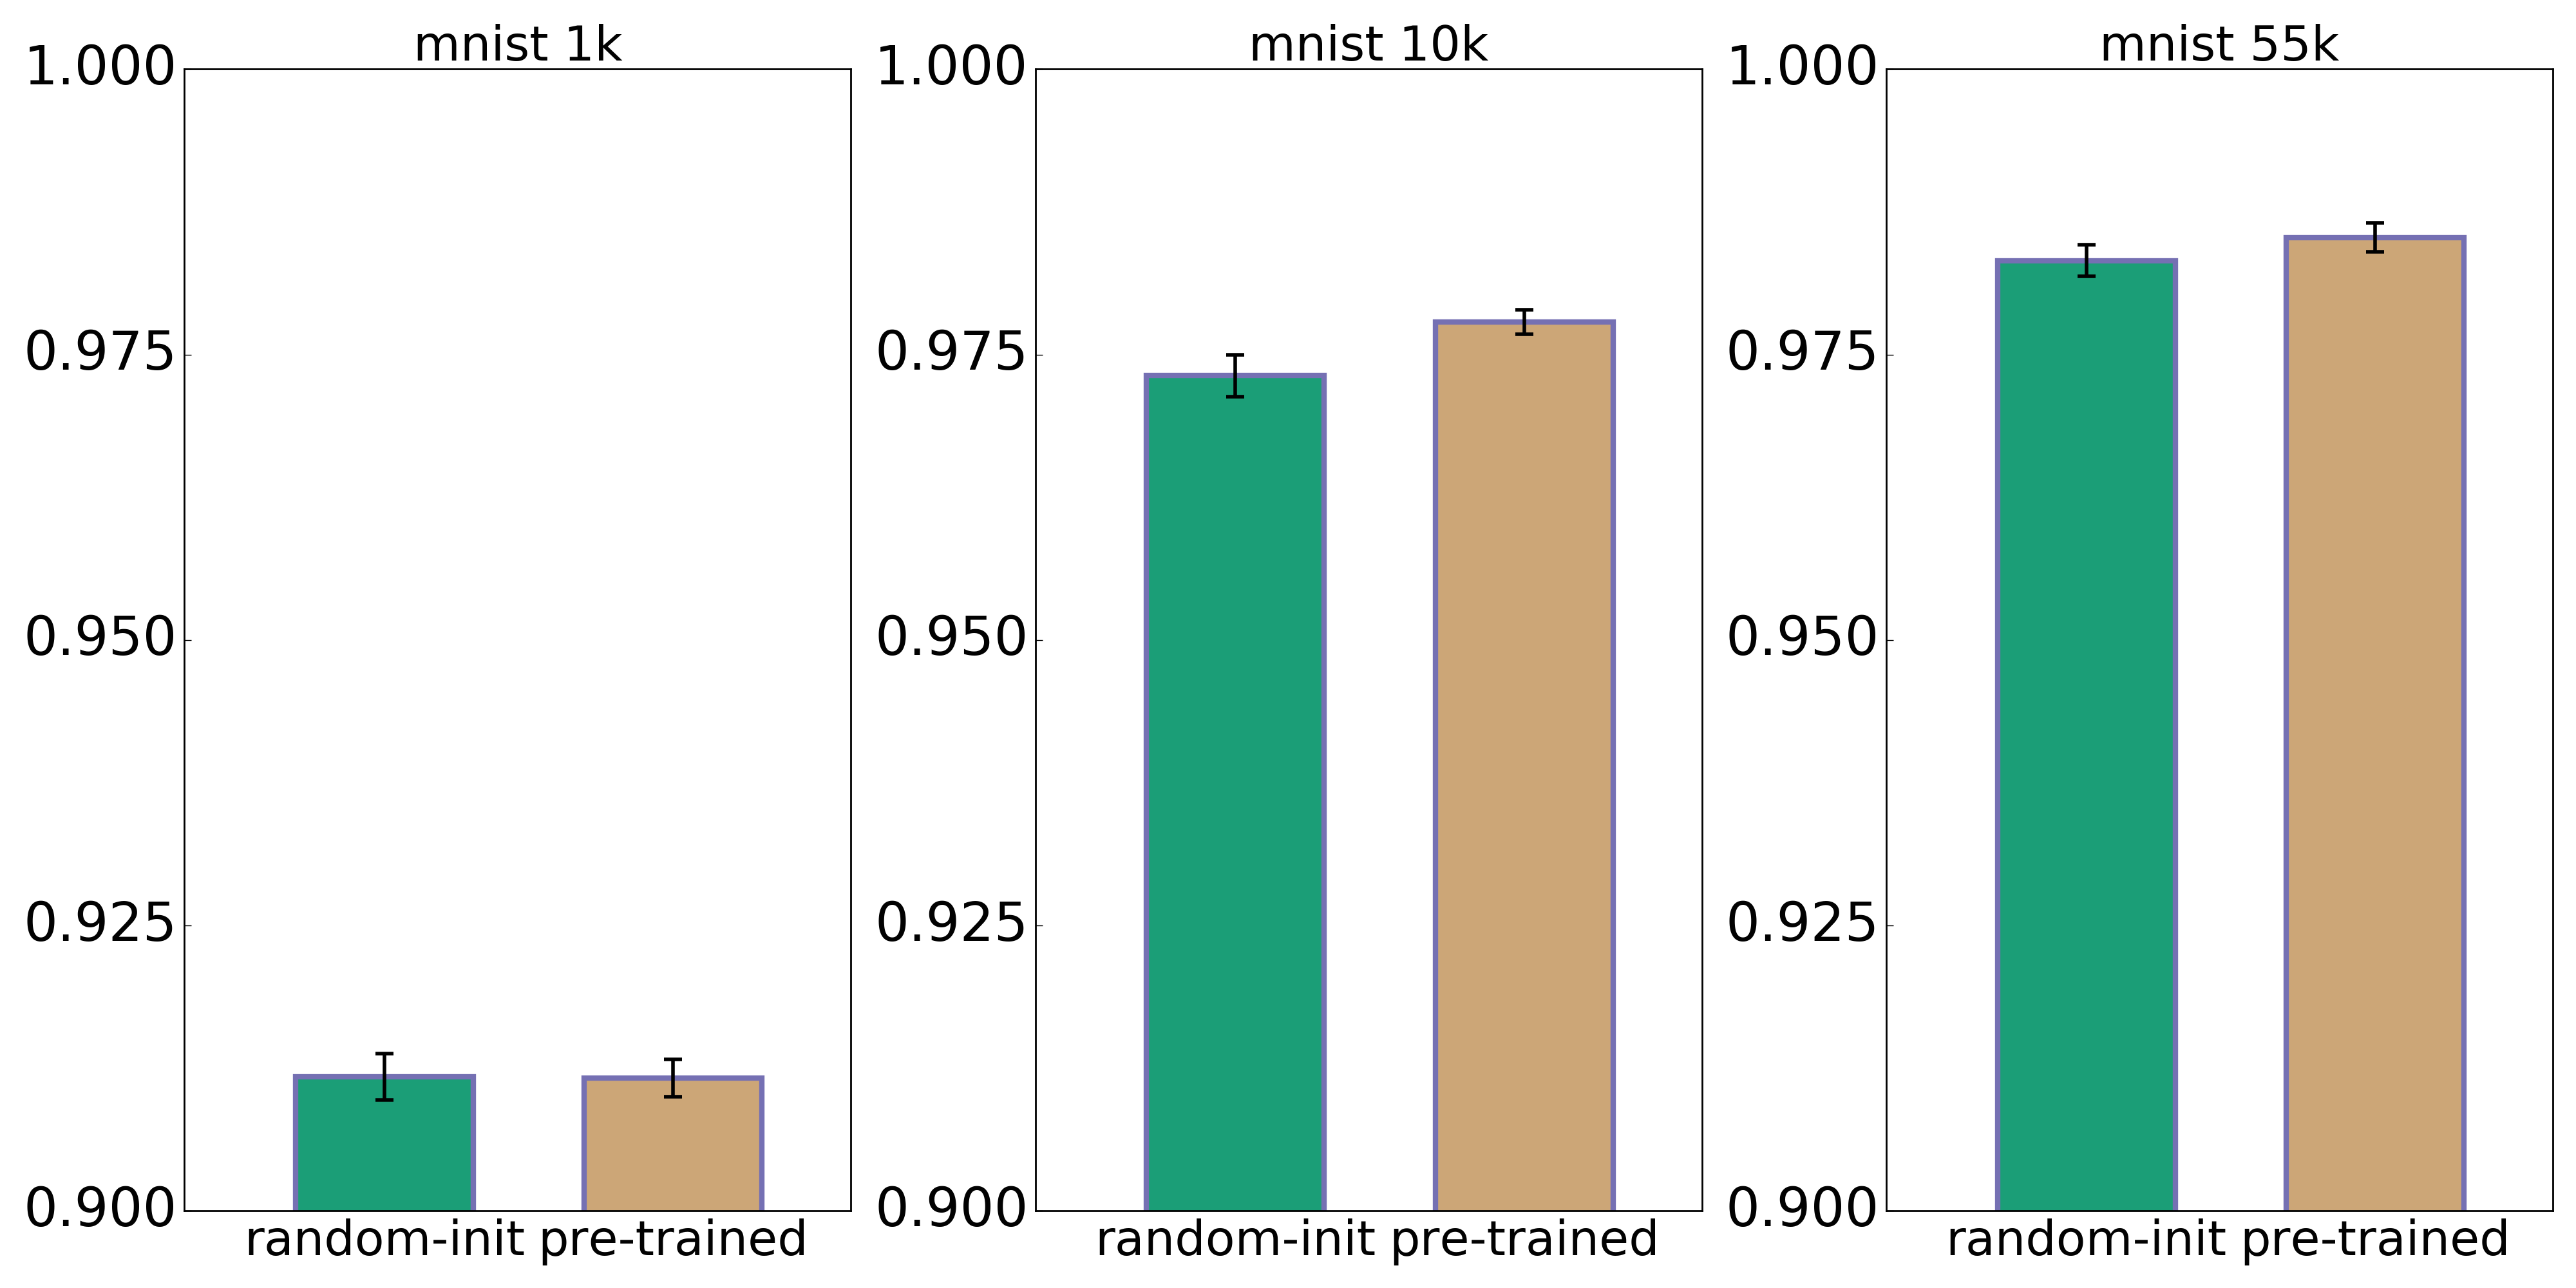
\includegraphics[width=\linewidth]{../box_plots/boxplots_mnist.png}
      \caption{\emph{MNIST}: test set accuracy comparison for different training set sizes (stddev in black)}
      \label{fig:mnist_plot}
    \end{figure}

    \begin{figure}
      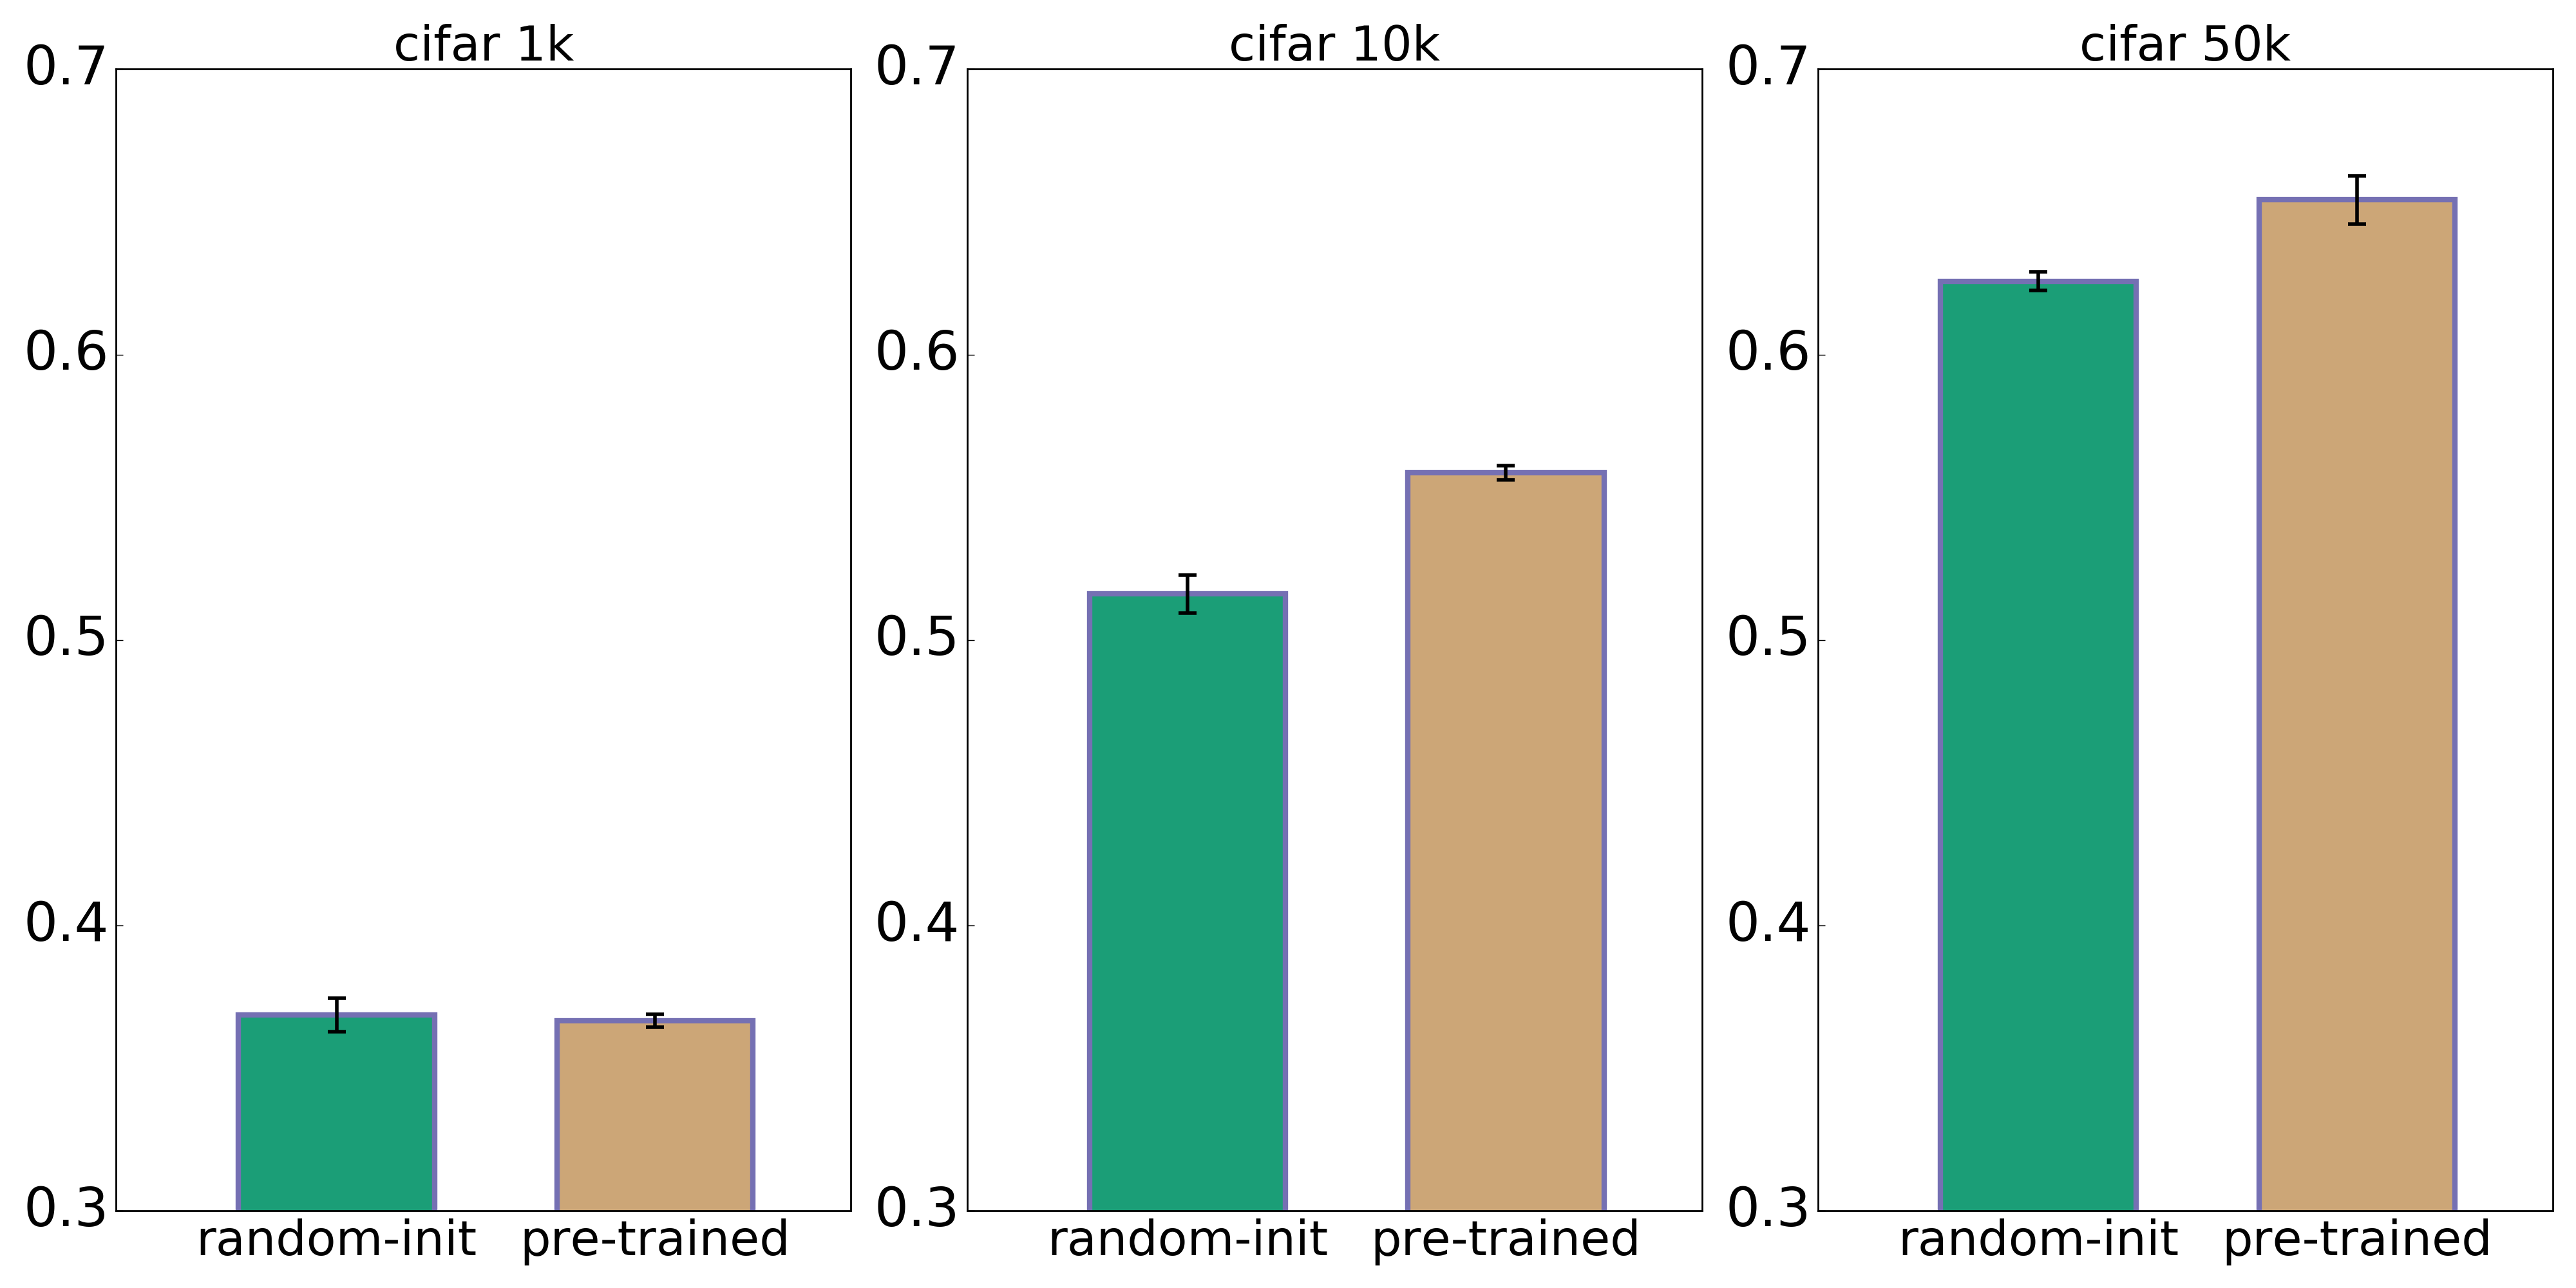
\includegraphics[width=\linewidth]{../box_plots/boxplots_cifar.png}
      \caption{\emph{CIFAR-10}: test set accuracy comparison for different training set sizes (stddev in black)}
      \label{fig:cifar_plot}
    \end{figure}

    \begin{figure}
      \centering
      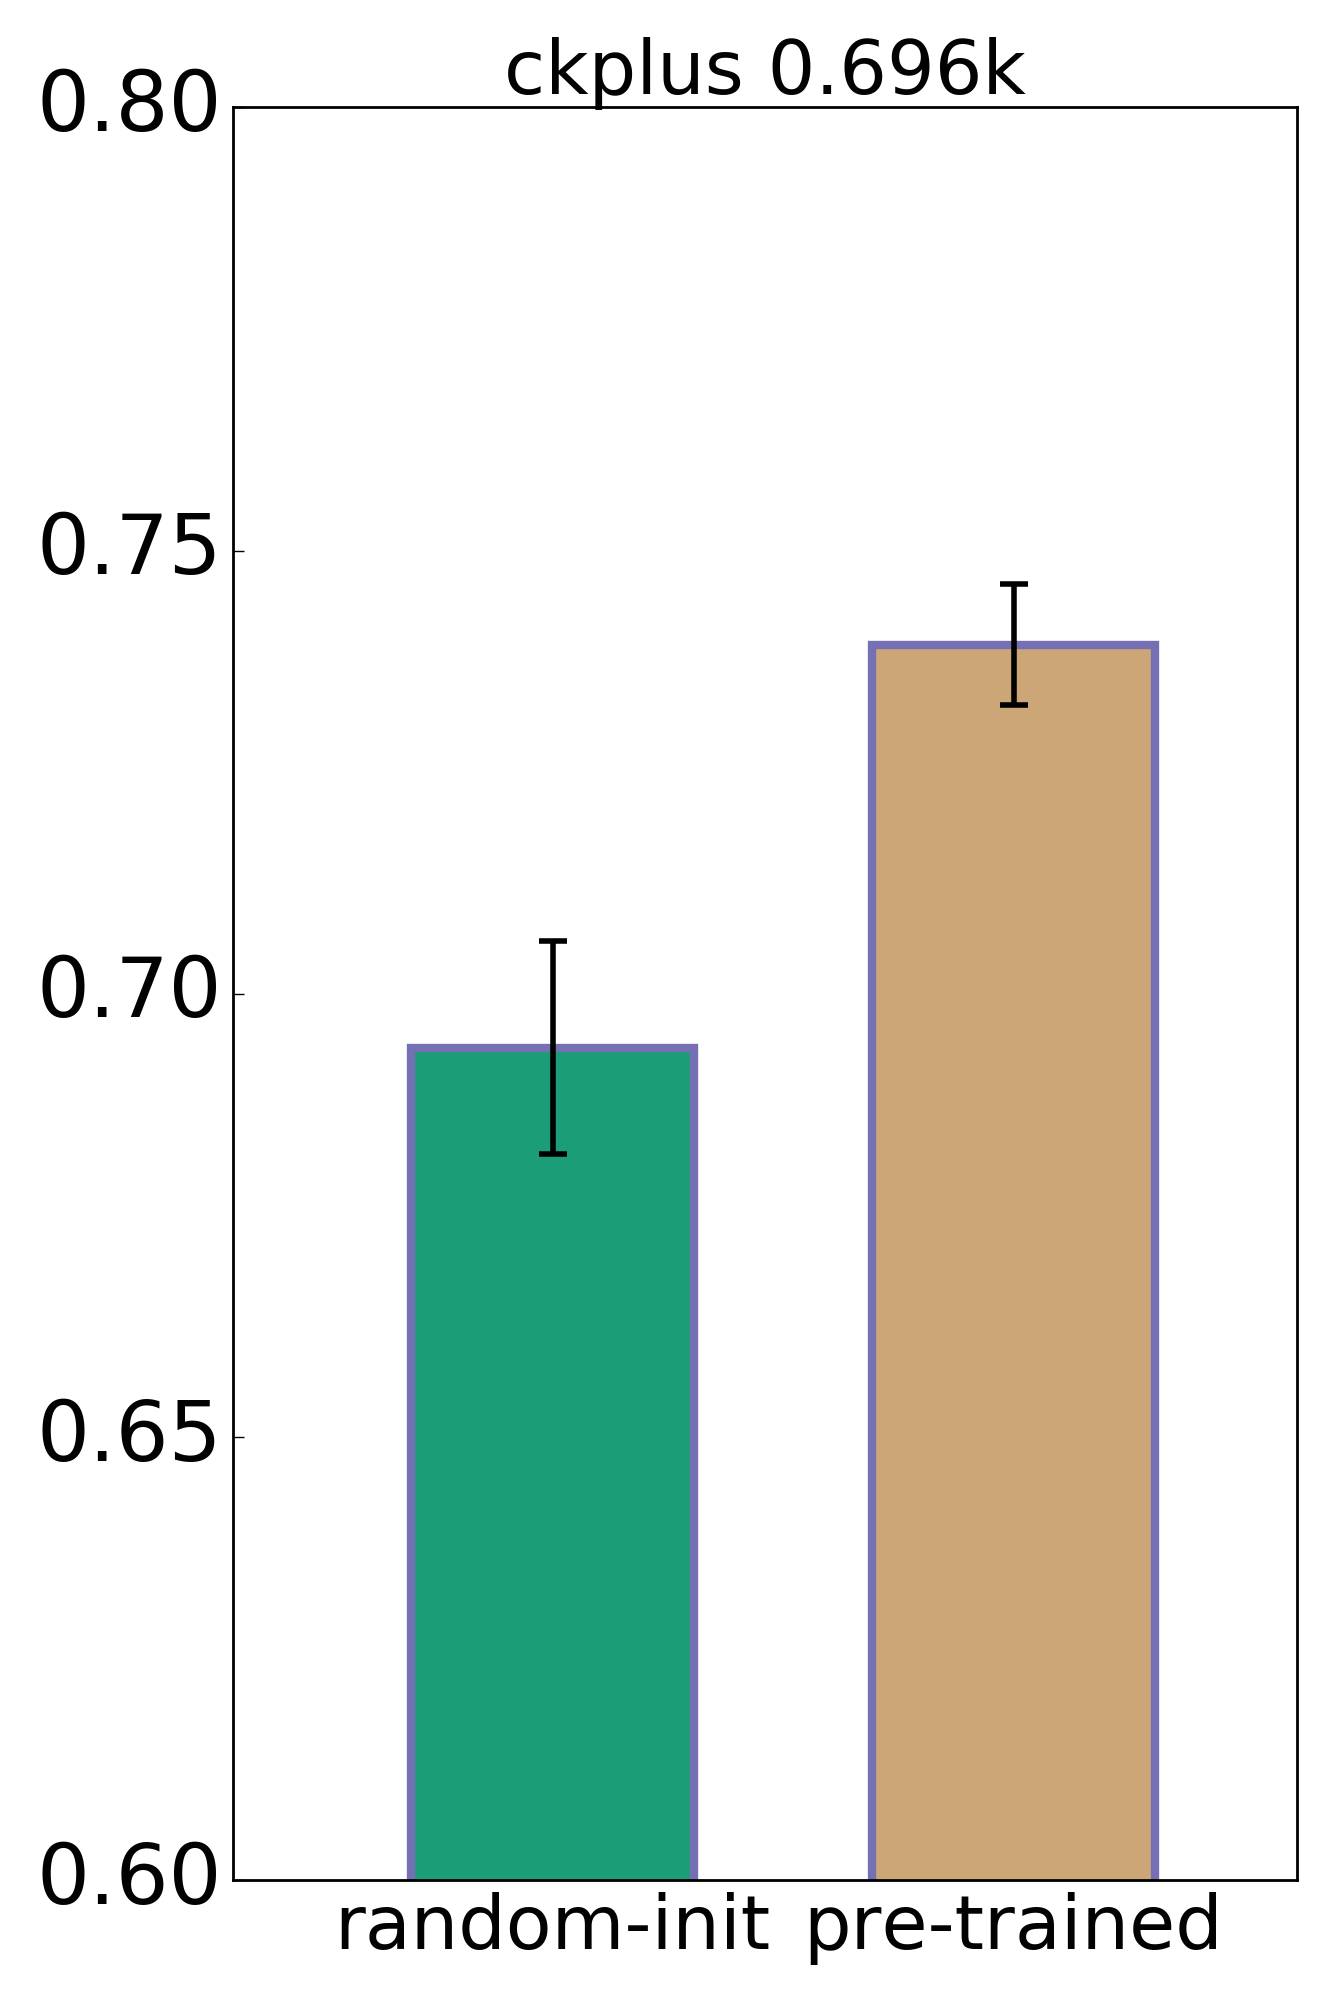
\includegraphics[width=0.33\linewidth]{../box_plots/boxplots_ckplus.png}
      \caption{\emph{CK+}: test set accuracy comparison for 696 training images (stddev in black)}
      \label{fig:ckplus_plot}
    \end{figure}

  \subsection{Statistical Significance}
    In order to check the statistical significance of the achieved pretraining improvements, we conducted the McNemar test. This way we calculated the probability (p-value) that the improvements could occur, when the pretrained network was not better than the randomly initialized one (Null-hypothesis).
    As can be seen in table \ref{table:significance}, the improvements for (...TODO...) are significant.
    \begin{table}
      \caption{Statistical Significance of Pretraining Improvements}
      \label{table:significance}
      \centering
      \begin{tabular}{lll}
        \toprule
        %\multicolumn{2}{c}{Part}                   \\
        %\cmidrule{1-2}
        Dataset     & Size     & Significance (p-value) \\
        \midrule
        MNIST & 1k  &     \\
        & 10k  &      \\
        & 50k  &     \\
        \midrule
        CIFAR-10     & 1 &     \\
        & 10 &      \\
        & 50k &      \\
        \midrule
        CK+     & 1k      &  \\
        \bottomrule
      \end{tabular}
    \end{table}


\section{Discussion and Conclusion}
  
  \begin{itemize}

    \item Evaluation of the Results         (Does it work)
    \item Evaluation of further experiments (When does it work, comparison with relu etc)

  \end{itemize}

\clearpage
\bibliography{references}

\end{document}
